\section{パーセプトロン}
\subsection{パーセプトロンとは}
パーセプトロンとは,複数の信号を入力として受けとり,1つの信号を出力する.ここでいう「信号」とは,電流や川のような「流れ」をもつものをイメージするとよいでしょう.電流が同線を流れ,電子を先に送り出すように,パーセプトロンの信号も流れを作り,情報を先へと伝達していきます.たあし,実際の電流とは違い,パーセプトロンの信号は「流す/流さない(1か0)」の二値の値です.本書では,0を「信号を流さない」1を「信号を流す」に対応させて記述します.
さて、\fref{fig:perceptron2}には、2つの信号を入力として受け取るパーセプトロンの例を示しています。$x_1$、$x_2$は入力信号、$y$は出力信号、$w_1$、$w_2$は重みを表します。図の〇は「ニューロン」や「ノード」と呼ばれます。入力信号は、ニューロンに送られる際に、それぞれに固有の重みが乗算されます。ニューロンでは、送られてきた信号の総和が計算され、その総和がある程度限界値を超えた場合にのみ1を出力します。これを「ニューロンが発火する」と表現することもあります。ここでは、その限界値を\textbf{閾値}と呼び、$\theta$という記号で表すことにします。以下にパーセプトロンの動作原理を示します.

\begin{figure}[h]
  \vspace{0mm}
  \begin{center}
    \hspace{0mm}
    \centering
    \includegraphics[width=30mm]{Ch2/peceptron2.png} \
    \vspace{0mm}
    \caption{2入力のパーセプトロン.}
    \label{fig:perceptron2}
  \end{center}
\end{figure}


\begin{equation}
    y = \left\{
\begin{array}{ll}
0 & (b + \omega_1 x_1 + \omega_2 x_2 \le 0)\\
1 & (b + \omega_1 x_1 + \omega_2 x_2 > 0)
\end{array}
    \right.
\end{equation}

\subsection{単純な論理回路}
\subsubsection{ANDゲート}
ANDゲートの真理値表を,\tref{tab:2_AND}に示す.
\begin{table}[htb]
    \centering
    \begin{tabular}{ccc}
        $x_1$ & $x_2$ & $y$ \\  % 1行目
        \hline
        \hline
        0 & 0 & 0 \\  % 2行目
        \midrule
        1 & 0 & 0 \\  % 3行目
        \midrule  % 太い線
        0 & 1 & 0 \\ 
        \midrule  % 太い線
        1 & 1 & 1 \\
        \end{tabular}
    \caption{ANDゲートの真理値表}
    \label{tab:2_AND}
\end{table}

\subsubsection{NANDゲートとORゲート}
NANDゲートとORゲートの真理値表を\tref{tab:2_NAND},\tref{tab:2_OR}に示す.
\begin{table}[htb]
    \centering
    \begin{tabular}{ccc}
        $x_1$ & $x_2$ & $y$ \\  % 1行目
        \hline
        \hline
        0 & 0 & 1 \\  % 2行目
        \midrule
        1 & 0 & 1 \\  % 3行目
        \midrule  % 太い線
        0 & 1 & 1 \\ 
        \midrule  % 太い線
        1 & 1 & 0 \\
        \end{tabular}
    \caption{NANDゲートの真理値表}
    \label{tab:2_NAND}
\end{table}

\begin{table}[htb]
    \centering
    \begin{tabular}{ccc}
        $x_1$ & $x_2$ & $y$ \\  % 1行目
        \hline
        \hline
        0 & 0 & 0 \\  % 2行目
        \midrule
        1 & 0 & 1 \\  % 3行目
        \midrule  % 太い線
        0 & 1 & 1 \\ 
        \midrule  % 太い線
        1 & 1 & 1 \\
        \end{tabular}
    \caption{ORゲートの真理値表}
    \label{tab:2_OR}
\end{table}

\subsection{パーセプトロンの実装}
\subsubsection{簡単な実装}
ANDゲートの実装を\lref{lst:AndGate.py}に示す.

\subsubsection{重みとバイアスの導入}
\begin{equation}
    y=f(x) = \left\{
\begin{array}{ll}
0 & (\omega_1 x_1 + \omega_2 x_2 \le \theta)\\
1 & (\omega_1 x_1 + \omega_2 x_2 > \theta)
\end{array}
    \right.
\end{equation}

\subsubsection{重みとバイアスによる実装}
NANDゲート,ORゲートの実装を\lref{lst:NandGate.py},\lref{lst:OrGate.py}に示す.
AND,NAND,ORは同じ構造のパーセプトロンであり,違いは重みパラメータの値だけ.

\subsection{パーセプトロンの限界}
これまで見てきたように,パーセプトロンを用いれば,AND,NAND,ORの3つの論理回路を実装することができました.それでは続いてXORゲートについて考えてみたいと思います.

\subsubsection{XORゲート}
XORゲートは排他的論理和とも呼ばれる論理回路です.\tref{tab:2_XOR}に示すように,$x_1$と$x_2$のどちらかが1の時だけ出力が1になります.(「排他的」とは自分以外は拒否することを意味します).さて,このXORゲートをパーセプトロンで実装するには,どのような重みパラメータを設定すればよいでしょうか?
実は,これまで見てきたパーセプトロンでは,このXORゲートを実装することはできません.なぜANDやORは実現できて,XORは実現できないのでしょうか.それを説明するために,ここでは図を用いて説明します.以下の図では,0を〇,1を$\square$で表しています.OR
ゲートを作ろうと思えば,\fref{fig:2_OR_png}を直線によって分ける必要があります.実際,左記の直線は,4つの点を正しく分けることができています.
しかし,\fref{fig:2_XOR_png}を直線によって分けることは,いくら考えてもできないでしょう.実は,一本の直線では,〇と$\square$を分けることができないのです.


\begin{table}[htb]
    \centering
    \begin{tabular}{ccc}
        $x_1$ & $x_2$ & $y$ \\  % 1行目
        \hline
        \hline
        0 & 0 & 0 \\  % 2行目
        \midrule
        1 & 0 & 1 \\  % 3行目
        \midrule  % 太い線
        0 & 1 & 1 \\ 
        \midrule  % 太い線
        1 & 1 & 0 \\
        \end{tabular}
    \caption{XORゲートの真理値表}
    \label{tab:2_XOR}
\end{table}

\begin{figure}[htb]
    \vspace{0mm}
    \begin{center}
      \hspace{0mm}
      \centering
      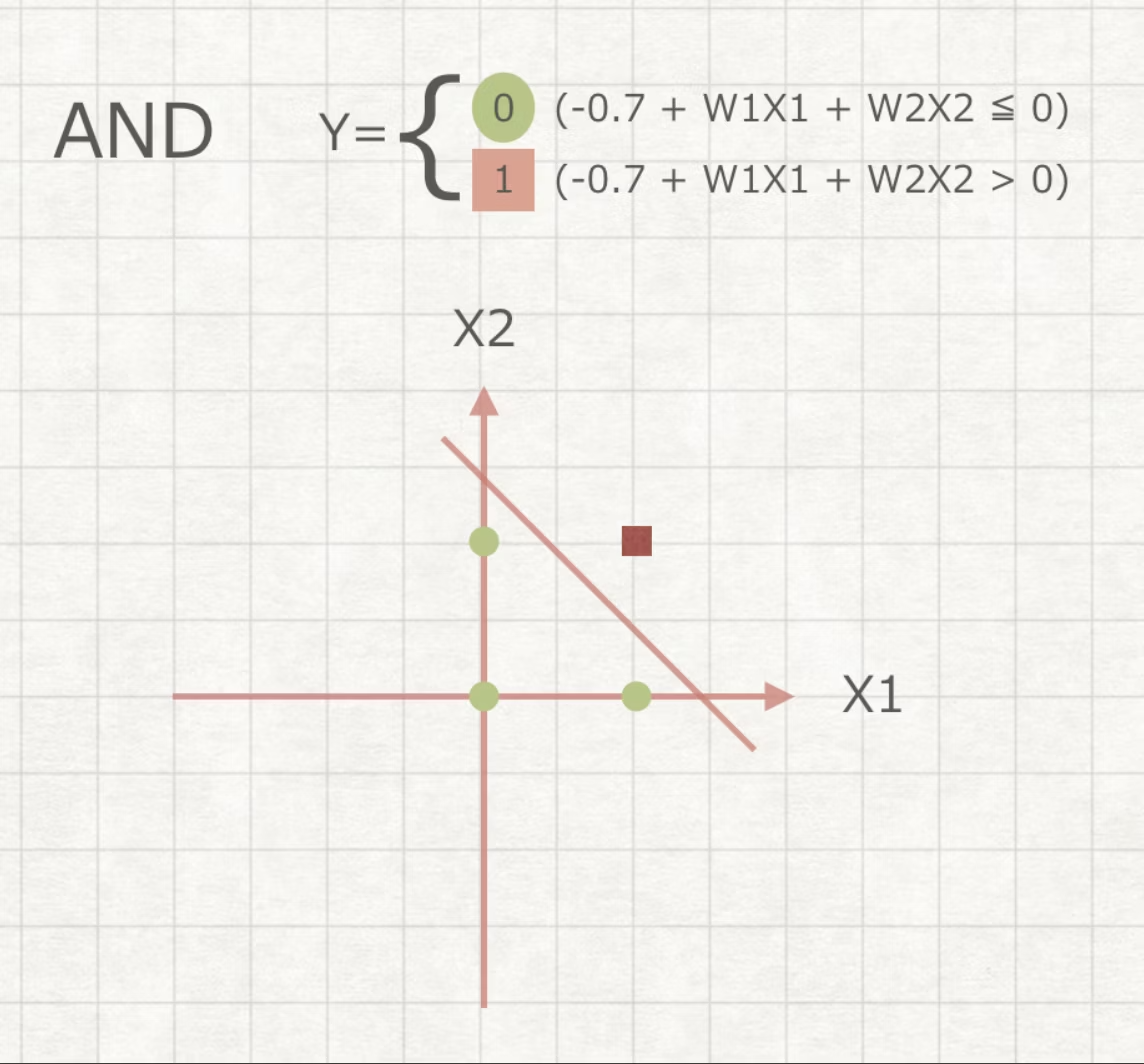
\includegraphics[width=65mm]{../1/Ch2/AND.png} \
      \vspace{0mm}
      \caption{2\_AND\_png}
      \label{fig:2_AND_png}
    \end{center}
  \end{figure}

  \begin{figure}[htb]
    \vspace{0mm}
    \begin{center}
      \hspace{0mm}
      \centering
      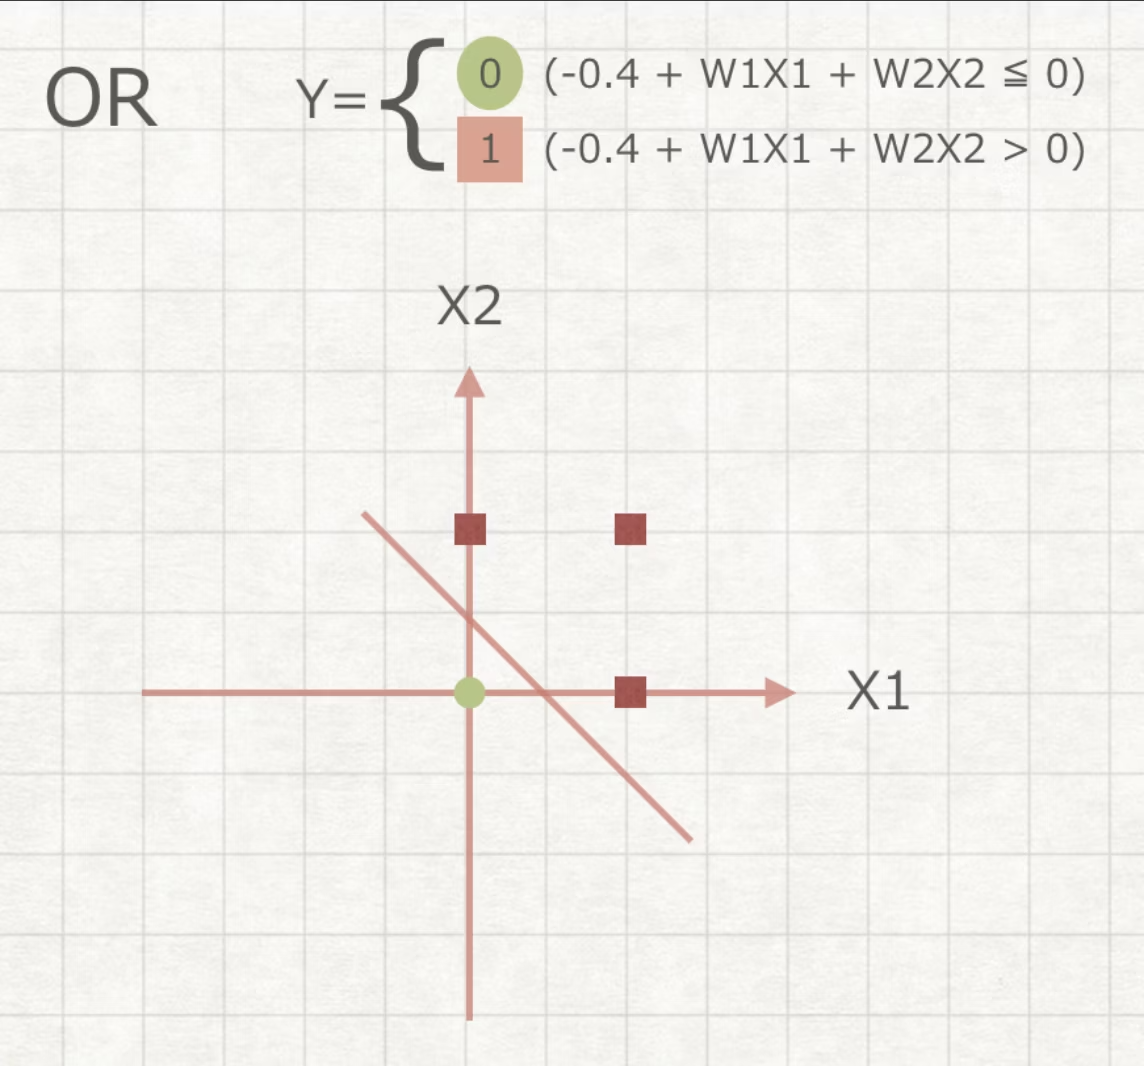
\includegraphics[width=65mm]{../1/Ch2/OR.png} \
      \vspace{0mm}
      \caption{fig:2\_OR\_png}
      \label{fig:2_OR_png}
    \end{center}
  \end{figure}

  \begin{figure}[htb]
    \vspace{0mm}
    \begin{center}
      \hspace{0mm}
      \centering
      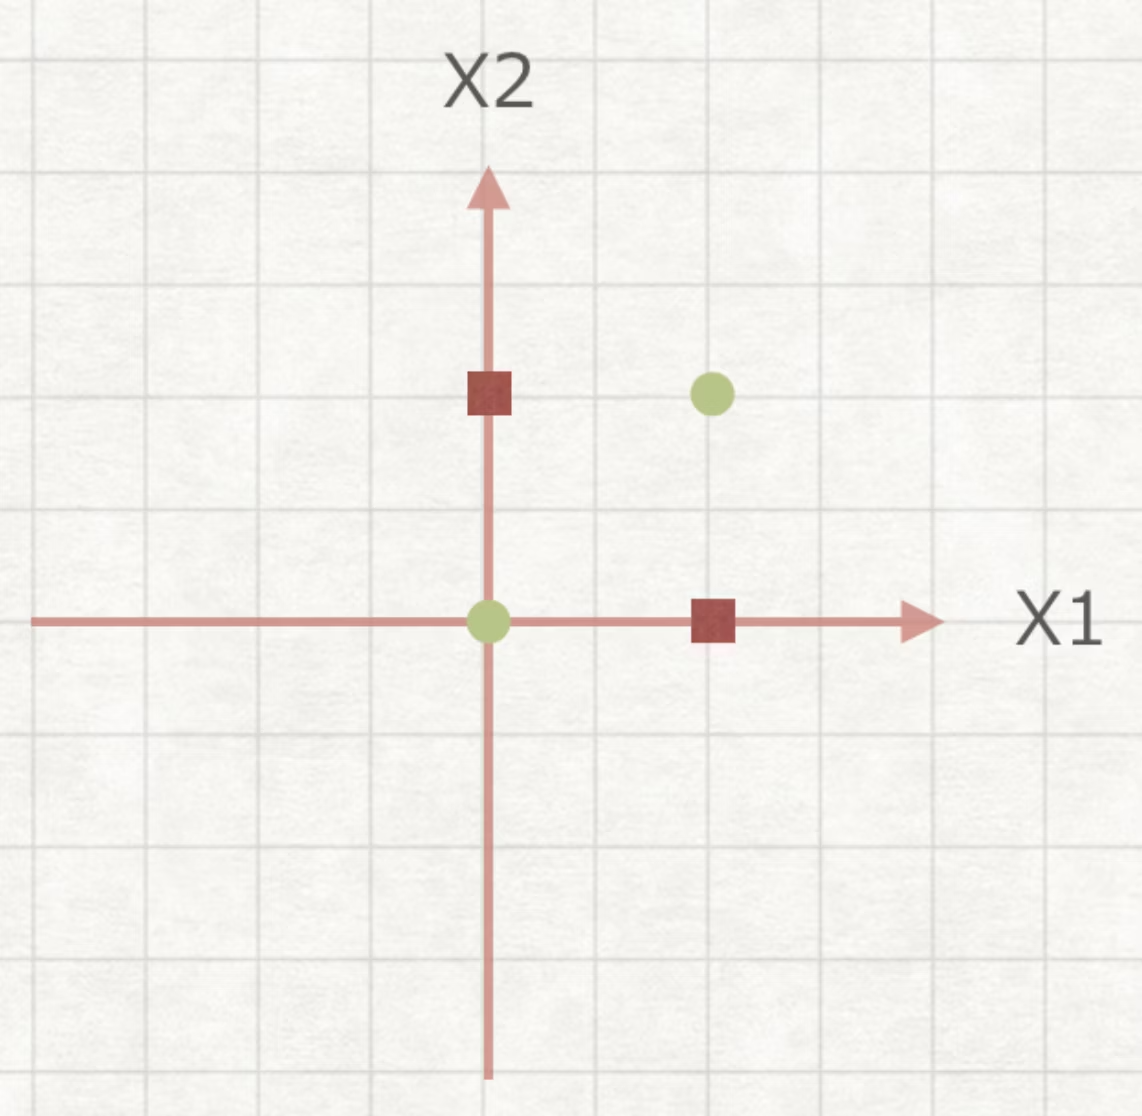
\includegraphics[width=65mm]{../1/Ch2/XOR.png} \
      \vspace{0mm}
      \caption{fig:2\_XOR\_png}
      \label{fig:2_XOR_png}
    \end{center}
  \end{figure}

\subsubsection{線形と非線形}
\fref{fig:2_XOR_png}の〇と$\square$は,一本の直線では分けることができません.しかし,もし"直線"という制約を外すことができたら,〇と$\square$を分けることができます.
\begin{figure}[htb]
    \vspace{0mm}
    \begin{center}
      \hspace{0mm}
      \centering
      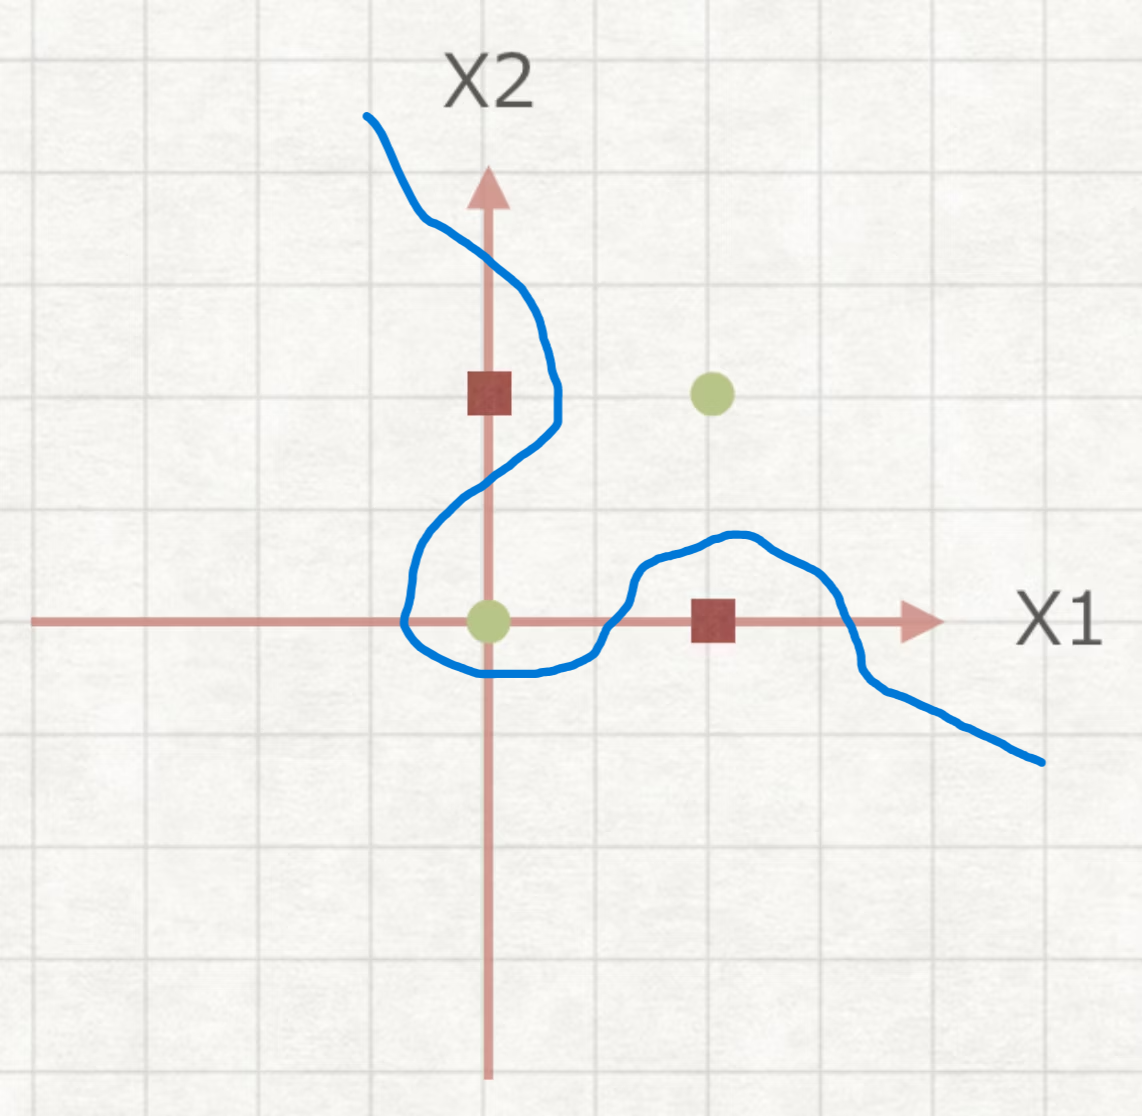
\includegraphics[width=65mm]{../1/Ch2/XOR2.png} \
      \vspace{0mm}
      \caption{fig:2\_XOR2\_png}
      \label{fig:2_XOR2_png}
    \end{center}
  \end{figure}

\subsection{多層パーセプトロン}
残念ながら,パーセプトロンはXORゲートを表現できませんでした.しかし,これは悲しいニュースではありません.実はパーセプトロンの素晴らしさは,"層を重ねる"ことができる点にあります(層を重ねることでXORを表現できるようになるというのが,本筋の筋書です).ここでは「層を重ねる」というのがどう言うことかという説明は後回しにして,XORゲートの問題を別の視点から考えたいと思います.
\subsubsection{既存ゲートの組み合わせ}
XORゲートを作るにはいくつか方法があるが,その一つにAND,NAND,ORゲートを組み合わせる方法がある.XORゲートは教科書の図2-11で実現することができる.\footnote{前節で述べたパーセプトロンの限界は,正確に言うと,「単層のパーセプトロンではXORゲートを表現できない」または「単層のパーセプトロンでは非線形領域は分離できない」ということになります.これから,パーセプトロンを組み合わせることで(層を重ねることで),XORゲートを表現できることを見ていきます.}

\begin{figure}[h]
  \vspace{0mm}
  \begin{center}
    \hspace{0mm}
    \centering
    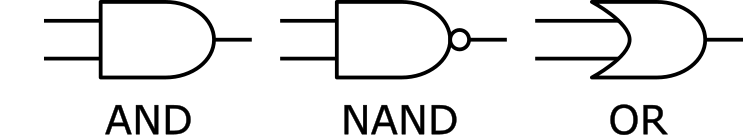
\includegraphics[width=70mm]{Ch2/path13.png} \
    \vspace{0mm}
    \caption{キャプション.}
    \label{fig:ラベル}
  \end{center}
\end{figure}

\begin{figure}[h]
  \vspace{0mm}
  \begin{center}
    \hspace{0mm}
    \centering
    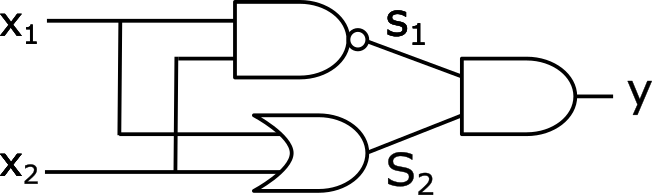
\includegraphics[width=70mm]{Ch2/XOR_AND_NAND_OR.png} \
    \vspace{0mm}
    \caption{キャプション.}
    \label{fig:2_XOR_AND_NAND_OR}
  \end{center}
\end{figure}

\begin{table}[htb]
    \centering
    \begin{tabular}{cc|cc|c}
        $x_1$ & $x_2$ & $s_1$& $s_2$& $y$ \\  % 1行目
        \hline
        \hline
        0 & 0 & 1 & 0 & 0 \\  % 2行目
        \midrule
        1 & 0 & 1& 1& 1 \\  % 3行目
        \midrule  % 太い線
        0 & 1 & 1& 1& 1 \\ 
        \midrule  % 太い線
        1 & 1 & 0& 1& 0 \\
        \end{tabular}
    \caption{XORゲートの真理値表}
    \label{tab:2_XOR_AND_NAND_OR}
\end{table}

\subsubsection{XORゲートの実装}
XORゲートの実装を\lref{lst:XorGate.py}に示す.
XORは、\fref{fig:2_XOR_perceptron}に示すような多層構造のネットワークです。ここでは、一番左の段を第0層、その右の段を第1層、一番右の段を第2層と呼ぶことにします。

さて、\fref{fig:2_XOR_perceptron}のパーセプトロンは、これまで見てきたANDやORが単層のパーセプトロン(\fref{fig:perceptron2})とは異なる形をしています。実際、ANDやORが単層のパーセプトロンであったのに対して、XORは2層のパーセプトロンです。ちなみに、層を複数重ねたパーセプトロンを\textbf{多層パーセプトロン}ということがあります。

\fref{fig:2_XOR_perceptron}に示すような2層のパーセプトロンでは、第0層と第1層のニューロンの間で信号の送受信が行われ、続いて第1層と第2層の間で信号の送受信が行われます。この動作をより詳しく述べると、次のようになります。\footnote{    \fref{fig:2_XOR_perceptron}のパーセプトロンは合計で3層から構成されますが、重みを持つ層は実質2層(第0層と第1層の間、第1層と第2層の間)であるため、
「2層のパーセプトロン」と呼ぶことにします。}

\begin{enumerate}
    \item 第0層の2つのニューロンが入力信号を受け取り、第1層のニューロンへ信号を送る 
    \item 第1層のニューロンが第2層のニューロンへ信号を送り、第2層芽のニューロンは$y$を出力する
\end{enumerate}

\begin{figure}[h]
  \vspace{0mm}
  \begin{center}
    \hspace{0mm}
    \centering
    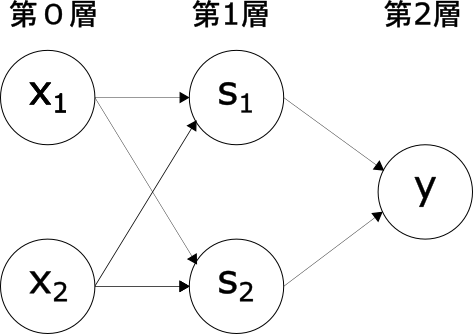
\includegraphics[width=50mm]{Ch2/XOR_perceptron.png} \
    \vspace{0mm}
    \caption{XORのパーセプトロンによる表記.}
    \label{fig:2_XOR_perceptron}
  \end{center}
\end{figure}

\subsection{NANDからコンピュータへ}
コンピュータの内部はとても複雑な処理を行っているように思えますが、実はNANDゲートの組み合わせだけで、コンピュータが行う処理を再現することができるのです。このことは、パーセプトロンでもコンピュータを表現できるということを意味しています。

\subsubsection{まとめ}
\begin{mdframed}[frametitle={本章で学んだこと}]
    \begin{itemize}
        \item パーセプトロンは入出力を備えたアルゴリズムである。ある入力を与えたら、決まった値が出力される。
        \item パーセプトロンでは、「重み」と「バイアス」をパラメータとして設定する。
        \item パーセプトロンを用いれば、AND、OR、NANDゲートなどの論理回路を表現できる。
        \item XORゲートは単層のパーセプトロンでは表現できない。
        \item 2層のパーセプトロンを用いれば、XORゲートを表現できる。
        \item  単層のパーセプトロンは線形領域だけしか分離できないが、多層のパーセプトロンは非線形領域も分離できる。
        \item 多層のパーセプトロンを用いれば、(理論上は)コンピュータが行う処理を再現できる。
    \end{itemize}
\end{mdframed}

\subsection{ソースコード}
2章のソースコードを以下に示します.
\ShowPython{AndGate.py}
\ShowPython{OrGate.py}
\ShowPython{NandGate.py}
\ShowPython{XorGate.py}
